\documentclass{article}
\usepackage
[
    a4paper,
    top=2cm,
    bottom=3cm,
    left=2cm,
    right=2cm
]{geometry}
\usepackage{amssymb}
\usepackage{amsmath}
\usepackage{array}
\usepackage{xeCJK}
\setCJKmainfont{微軟正黑體}

\title{自動機與形式語言 Homework 2}
\author{Class 02 B03902086 李鈺昇}
\date{}

\begin{document}
    \maketitle
    
    \section*{(1)(2)}
        \begin{tabular}{m{0.1\textwidth}|m{0.6\textwidth}|m{0.2\textwidth}}
            (a) & 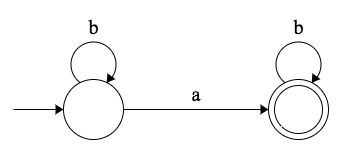
\includegraphics[width=0.3\paperwidth]{fig/a.png} & $b^*ab^*$ \\
            \hline
            (b) & 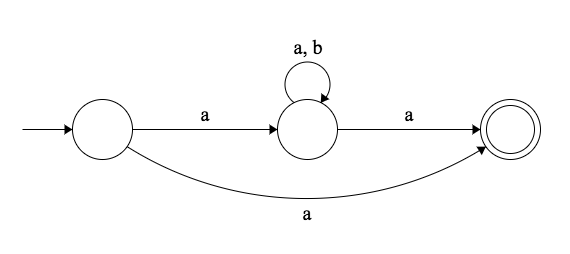
\includegraphics[width=0.4\paperwidth]{fig/b.png} & $a\Sigma^*a \cup a$ \\
            \hline
            (c) & 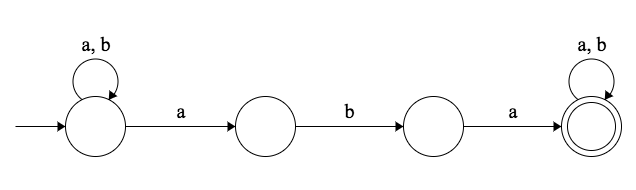
\includegraphics[width=0.4\paperwidth]{fig/c.png} & $\Sigma^*aba\Sigma^*$ \\
            \hline
            (d) & 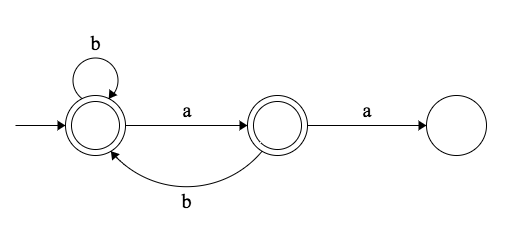
\includegraphics[width=0.4\paperwidth]{fig/d.png} & $(ab \cup b)^*(\epsilon \cup a)$ \\
            \hline
            (e) & 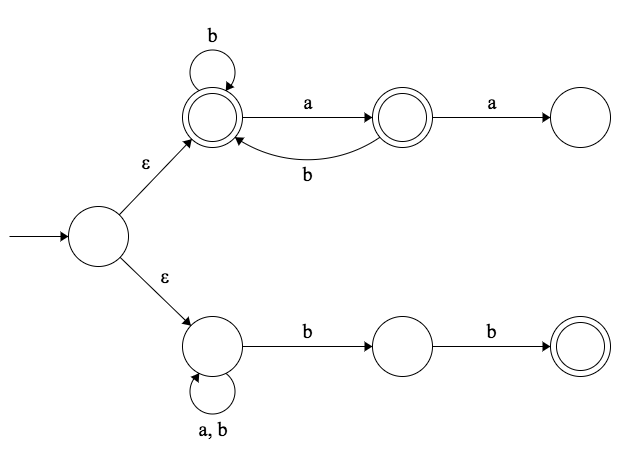
\includegraphics[width=0.4\paperwidth]{fig/e.png} & $(ab \cup b)^*(\epsilon \cup a) \cup \Sigma^*bb$
        \end{tabular}
    
    \linespread{2.0}

    \section*{(3)}
        \subsection*{(a)}
            Regular. Regex: $b^*ab^*ab^*ab^*$
            
        \subsection*{(b)}
            Regular. Regex: $(b^*ab^*ab^*)^*$
            
        \subsection*{(c)}
            Regular. Regex: $(\Sigma\Sigma)^*$
            
        \subsection*{(d)}
            Nonregular. \\
            Suppose $L$ is regular, and the pumping length is $p$.
            Take $s = a^pba^p \in L$.
            Clearly $|s| = 2p+1 \geq p$, and pumping lemma says that
            there exists $x, y, z$ such that
            $s = xyz, |y| > 0, |xy| \leq p, xy^iz \in L \; \forall i \geq 0$.
            Thus $y \neq \epsilon$ and y consists only of $a$'s. \\
            If we examine $xy^0z = xz$, then there would be fewer $a$'s on the
            left side of $b$ ($|y| > 0$), implying that $xz \notin L$.
            Hence $L$ is NOT regular.
            
        \subsection*{(e)}
            Nonregular. \\
            Suppose $L$ is regular, and the pumping length is $p$.
            Take $s = a^q \in L$,
            where $q \geq p$ is a chosen prime (possible since primes are unbounded).
            Clearly $|s| = q \geq p$, and pumping lemma says that
            there exists $x, y, z$ such that
            $s = xyz, |y| > 0, |xy| \leq p, xy^iz \in L \; \forall i \geq 0$.
            Thus $y \neq \epsilon$ and y consists only of $a$'s. \\ \\
            Now let $r = |x| + |z|$ and consider three cases:
            \begin{itemize}
                \item $r = 0$ \\
                In this case, $x = z = \epsilon$ and $|y| = q$.
                Examine $xy^qz = y^q$, whose length is $q^2$,
                not a prime ($q$ is a prime so $q > 1$).
                So $xy^qz \notin L$.
                
                \item $r = 1$ \\
                Examine $xy^0z = xz$, whose length is $|xz| = |x| + |z| = r = 1$,
                not a prime.
                So $xy^0z \notin L$.

                \item $r > 1$ \\
                Examine $xy^rz$,
                whose length is $|x| + r|y| + |z| = (|y| + 1)r$,
                not a prime ($|y| > 0$ so $|y| + 1 > 1$).
                So $xy^rz \notin L$.
            \end{itemize}
            In each case, pumping lemma fails, so $L$ is NOT regular.
    
    \section*{(4)}
        \subsection*{(a)}
            \begin{itemize}
                \item Reflexivity: Fix one $u \in \Sigma^*$. Now $\forall w \in \Sigma^*$,
                since trivially $uw = uw$, we immediately have $u \sim_L u$.
                
                \item Symmetry: $\forall u, v \in \Sigma^*$, \\
                $u \sim_L v$ \\
                $\Longrightarrow \forall w \in \Sigma^*, uw \in L$ iff $vw \in L$ \\
                $\Longrightarrow \forall w \in \Sigma^*, vw \in L$ iff $uw \in L$ \\
                $\Longrightarrow v \sim_L u$.
                
                \item Transitivity: $\forall x, y, z \in \Sigma^*$, \\
                $x \sim_L y$ and $y \sim_L z$ \\
                $\Longrightarrow \forall w \in \Sigma^*, xw \in L$ iff $yw \in L$ and $yw \in L$ iff $zw \in L$ \\
                $\Longrightarrow \forall w \in \Sigma^*, xw \in L$ iff $zw \in L$ \\
                $\Longrightarrow x \sim_L z$.
            \end{itemize}
        
        \subsection*{(b)}
            Suppose $u \sim_L v$.
            Take $w = \epsilon \in \Sigma^*$,
            then $uw = u$ and $vw = v$. \\
            By definition we know $u \in L$ iff $v \in L$,
            which implies either $u, v \in L$ or $u, v \notin L$.
        
        \subsection*{(c)}
            Assume $\mathcal{A} = \langle \Sigma, Q, q_0, F, \delta \rangle$. \\
            Suppose $u, v \in \Sigma^*$ with
            $\mathcal{A}(u) = \mathcal{A}(v) = q$ for some $q \in Q$.
            Then we consider the two possible cases:
            \begin{itemize}
                \item $q \in F$ \\
                In this case, both $u$ and $v$ are accepted by $\mathcal{A}$,
                so $u, v \in L$.
                
                \item $q \notin F$ \\
                In this case, both $u$ and $v$ are rejected by $\mathcal{A}$,
                so $u, v \notin L$.
            \end{itemize}
            Thus $u \in L$ iff $v \in L$, that is, $u \sim_L v$.
        
        \subsection*{(d)}
            Let $n = |Q|$. Suppose $\#(\sim_L) > n$,
            then there are at least $n + 1$ words
            $s_1, s_2, \dots, s_{n+1}$ such that $s_i \not\sim_L s_j, i \neq j$.
            From (c) we can conclude that for $u, v \in \Sigma^*$,
            if $u \not\sim_L v$, then $\mathcal{A}(u) \neq \mathcal{A}(v)$.
            So $s_1, \dots, s_{n+1}$ satisfies
            $\mathcal{A}(s_i) \neq \mathcal{A}(s_j), i \neq j$,
            which means that their are $n + 1$ distinct states.
            But $\mathcal{A}$ has only $n$ states, a contradiction.
            So $\#(\sim_L)$ is finite,
            and more specifically $\#(\sim_L) \leq n = |Q|$.
        
    \section*{(5)}
        \subsection*{(a)}
            Let $M = \{1, \dots, m\}$.
            For each $i \in M$, take one arbitrary word $s_i \in C_i$.
            Then let $S = \{i | s_i \in L\} \subseteq M$.
            Now I shall show that $L = \bigcup_{i \in S}{C_i}$. \\ \\
            On one hand, pick any $s \in L$, clearly $s \in C_j$ for some $j \in M$,
            since $\sim_L$ partitions $\Sigma^* \ni s$.
            Also $s_j \in C_j$, hence $s_j \sim_L s$. 
            By (4)(b) and $s \in L$, we know $s_j \in L$.
            So $j \in S$ by definition of $S$,
            hence $s \in C_j \subseteq \bigcup_{i \in S}{C_i}$. \\
            Since the above holds for all $s \in L$,
            we have $L \subseteq \bigcup_{i \in S}{C_i}$. \\ \\
            On the other hand, pick any $s \in \bigcup_{i \in S}{C_i}$.
            Then $s \in C_j$ for some $j \in S$.
            By $j \in S$ and my definition of $S$, $s_j \in L$.
            We already know $s_j \in C_j$, so again $s_j \sim_L s$.
            With $s_j \in L$ and (4)(b), $s \in L$. \\
            Since the above holds for all $s \in \bigcup_{i \in S}{C_i}$,
            we have $\bigcup_{i \in S}{C_i} \subseteq L$. \\ \\
            Now rewrite $S = \{i_1, \dots, i_k\}$ where $k = |S|$.
            Hence $L = \bigcup_{i \in S}{C_i} = C_{i_1} \cup \cdots \cup C_{i_k}$.
            This completes the proof.
        
        \subsection*{(b)}
            $\forall w_1, w_2 \in C_i, w_1 \sim_L w_2$,
            which by definition guarantees that
            $w_1x \in L$ iff $w_2x \in L$ for all $x \in \Sigma^*$.
            This implies $w_1ax \in L$ iff $w_2ax \in L$ for all $x \in \Sigma^*$.
            Again by definition, $w_1a \sim_L w_2a$,
            and thus $[w_1a] = [w_2a]$. \\
            Because the above holds for any $i$, the proof is done.
        
        \subsection*{(c)}
            \textbf{Claim \quad} For $s \in \Sigma^*, \mathcal{A}(s) = p_j$ if and only if
            $s \in C_j, 1 \leq j \leq m$.
            \begin{itemize}
                \item \textit{Proof: \quad}
                The proof is by induction on $|s|$. \\
                Base case, $|s| = 0$: So $s = \epsilon, \mathcal{A}(s) = q_0 = p_j$,
                where $s = \epsilon \in C_j$ as in the definition of $\mathcal{A}$. \\
                Now suppose the claim holds for all $s$ with $|s| = n, n \geq 0$.
                Then for any $s$ with $|s| = n+1$, say $s = s_1 s_2 \cdots s_{n+1}$,
                we know the claim holds for $s_1 \cdots s_n$.
                So we can assume $\mathcal{A}(s_1 \cdots s_n) = p_i$ and
                $s_1 \cdots s_n \in C_i$ for some $1 \leq i \leq m$.
                As in the definition of $\delta$, take $w = s_1 \cdots s_n \in C_i$
                and $a = s_{n+1}$, then $\delta(p_i, s_{n+1}) = p_j$ and
                $[s] = [s_1 \cdots s_n s_{n+1}] = C_j$ for some $1 \leq j \leq m$.
                Thus $\mathcal{A}(s) = \delta(\mathcal{A}(s_1 \cdots s_n), s_{n+1})
                = \delta(p_i, s_{n+1}) = p_j$ and $s \in C_j$.
                This induction step completes the proof.
            \end{itemize}
            Now we can work on the two directions of the problem.
            \begin{itemize}
                \item $L(\mathcal{A}) \subseteq L$ \\
                For any $s = s_1 s_2 \dots s_n \in L(\mathcal{A})$, there is a run
                $p_{j_0} s_1 p_{j_1} \dots s_{n-1} p_{j_{n-1}} s_n p_{j_n}$
                with $\epsilon \in C_{j_0}$ and $\mathcal{A}(s) = p_{j_n} \in F$.
                With the above claim, we can conclude $s = \in C_{j_n}$.
                And $p_{j_n} \in F = \{p_{i_1}, \dots, p_{i_k}\}$,
                so $j_n \in \{i_1, \dots, i_k\}$,
                hence $s \in C_{i_1} \cup \cdots \cup C_{i_k} = L$.
                
                \item $L \subseteq L(\mathcal{A})$ \\
                Suppose $s \in L = C_{i_1} \cup \cdots \cup C_{i_k}$.
                Then $s \in C_i$ for some $i \in \{i_1, \dots, i_k\}$.
                With the claim, $\mathcal{A}(s) = p_i \in \{p_{i_1}, \dots, p_{i_k}\} = F$.
                Hence $\mathcal{A}$ accepts $s$, or $s \in L(\mathcal{A})$.
            \end{itemize}
            This completes the proof.
            
        \subsection*{(d)}
            If $L$ is regular, then some DFA $\mathcal{A}$ recognizes it,
            and thus $\#(\sim_L) \leq |Q| < \infty$ by (4.d),
            where $Q$ is the set of states of $\mathcal{A}$. \\
            On the other hand, if $\#(\sim_L) = m < \infty$, then
            by the previous (5.abc) we can construct a DFA $\mathcal{A}$
            with $m$ states such that $L(\mathcal{A}) = L$, implying $L$ is regular.
\end{document}